\subsubsection{Use Case, Elaboration and Activity Diagram of Reviewing Comments}
One of the most important features of EvaP is the ability to review comments before publishing the results. 
This allows the responsibles to prevent hurtful and deconstructive comments from being visible to the lecturers.
Even more, the responsibles can change the comment in a way that the lecturer still receives the criticism.
This is the reason for the course state \emph{comment review pending}.
The described use case is documented in German on the Github wiki mentioned above 
(\url{https://github.com/fsr-itse/EvaP/wiki/Use-Case%3A-Review-Comments}).

Following is the use case elaboration translated, updated and adapted to the template presented in the lecture (Table \ref{tab:use-case}).
The activity diagram (Graphic \ref{fig:activity-diagram}) used to explore scenario testing and to create test cases is based on this elaboration.

\begin{table}[]
    \centering
    \label{tab:use-case}
    \begin{tabularx}{\textwidth}{|l|X|}
        \hline
        Use Case Name                      
            & Review Comments       \\ \hline 
        Summary                           
            & Student representatives review comments for violation of comment rules before publishing course results                \\ \hline
        Actor 
            & Student representatives (FSR)         \\ \hline
        Precondition          
            & A course has been evaluated and entered the state \emph{comment review pending} \\ \hline
        Description               
            & 	\begin{enumerate}
                    \item FSR opens list with comments of a course
                    \item FSR evaluates comments regarding the comment rules
                    \item FSR accepts all comments and marks them as \emph{publishing: yes}
                    \item FSR receives a small notices as the mark turns from white to green and fades back to a gray
                \end{enumerate}          \\ \hline
        Alternatives                 
            & 	\begin{enumerate}
                    \setcounter{enumi}{2}
                    \item FSR rejects one or more comments and marks them as \emph{publishing: no}
                \end{enumerate}
                \begin{enumerate}
                    \setcounter{enumi}{2}
                    \item FSR rejects one or more comments  and edits the comments before marking them as \emph{publishing: yes}
                \end{enumerate}
                \begin{enumerate}
                    \setcounter{enumi}{2}
                    \item FSR marks one or more comments and marks them as \emph{publishing: private} if they should only be visible to the specific tutor not all lecturers
                \end{enumerate}     \\ \hline
        Postcondition        
            & All comments marked as \emph{publishing: yes} or \emph{publishing: private} comply with the comment rules         \\ \hline
    \end{tabularx}
    \caption{Use case elaboration of reviewing comments}
\end{table}

%Created with https://www.draw.io/
\begin{figure}[h]
    \centering
    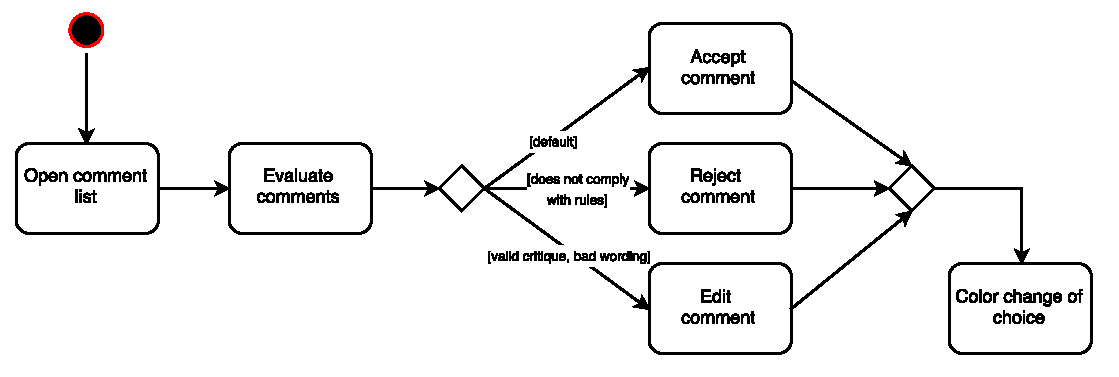
\includegraphics[width=\textwidth, keepaspectratio]{graphics/use-case}
    \caption{Activity diagram of the use case \emph{Review Comments}} %TODO state names
    \label{fig:activity-diagram}
\end{figure}

\paragraph{Scenario Testing --- Application: Learn the Product}
As a student representative you are responsible for supervising the evaluation process.
This includes reviewing all comments and validate their compliance with the comment rules.
After a course in evaluation enters the state \emph{comment review pending} open the list with comments.
They are arranged in groups according to the question answered.
For each comment read it carefully and evaluate its compliance with the comment rules.
Is the comment constructive critique? 
Could its content hurt the lecturers? 
Is it about a specific lecturer and could it be harmful if another lecturer read it?
Depending on your evaluation mark the comment as either \emph{publishing: yes}, \emph{publishing: no} or \emph{publishing: private}.
Observe the color change of your choice from white to green and its fading to grey.
This will help to ensure that you did not accidently mark the wrong choice.

\paragraph{Scenario Testing --- Experience Review}
While writing the testing scenario above we noticed that its application, in our case to learn the product, limits its use.
This testing scenario is useful for testers and eventually new users.
But, in comparison to coded tests, there is no automatic run of the scenario testing possible, respectively no automatic evaluation of a test run is possible.
Therefore, there is no automatic feedback to the developer if the scenario is still operable after changes to the code.
Furthermore, there is no direct evaluation available to the manager who normally can view a green light if all automatic tests run through.

Additionally, we noticed a few risks involved with relying on scenario testing.

A scenario involves several features that are even based on each other.
If a tester is not able to work through a scenario, the reason might not be obvious.
A tester might not be able to know which of the involved features failed.
A scenario testing might not always help with locating a bug.

It is thinkable that a testing scenario exposes design errors rather than code errors.
In our example the tester might wonder why there are not all three options \emph{yes, no, private} available for a comment. 
To find the reason you need the knowledge that the comment answered a generic question instead of a question tailored to a specific lecturer.
That the knowledge is not obvious on the webpage but needed as background knowledge, could be seen as a design error.
The code however does not contain this as an error.

As a software project has only limited resources available it is a risk to rely on scenario testing.
Since a tester runs the scenario testing, repetition of testing the same scenario is expensive.
Furthermore, repetition of a scenario testing could be unnecessary.
Communication between developers and testers is essential to avoid repeating a scenario testing after no changes influencing the features were made.
And after several repetitions a variation of the testing scenario might be preferable as it could detect bugs not covered by the previous run.

While scenario testing definitely has a very specific use and purpose it was pretty fun to write a hypothetical story to help a tester work through the use case.
It is an obviously creative way to generate tests for a software.
This allows it to ease the daily routine of a developer/tester.
Additionally, following a story allows a better insight into the system than following the manual.
It is in man's nature to love stories.

\paragraph{Test Cases}
There is no unit test for the actual code that offers the three marking options to the student representatives while reviewing comments.
The source code lies in \texttt{evap/staff/views.py} in the function \texttt{course\_comments\_update\_publish()}.
But following the use case we added a test, that checked if a marking is saved correctly in the model in \texttt{evap/staff/tests.py}.
There are already tests that check whether a comment marked as private is visible to an unauthorized result viewer in \texttt{evap/results/tests.py}.

Even though it would be pleasant to have a test case covering the offering of the three options and the marking, the more important part of this use case, the decision, can not be tested.
As the activity diagram shows a critical part is the decision, if a comment is to be marked as \emph{publishing: yes}, \emph{publishing: no} or \emph{publishing: private}.
At the moment this decision has to be made by the student representatives.
Even the student representative do not have documented guidelines for their decision.
Currently, it is based loosely on the aspect of constructive critique and empathy.

We can imagine that in the future an assistant system could help with the decision.
The default decision could be to publish comments as most comments are published at the current time.
Based on wording it could suggest to not publish comments containing swearwords.
Such a system could not only be used to help with the decision but also with checking decisions made.
It could highlight comments marked different from the suggestions.
Such a system would allow some tests regarding the presented use case.
%TODO so important, but no test case - very sad, much bad
